% Options for packages loaded elsewhere
\PassOptionsToPackage{unicode}{hyperref}
\PassOptionsToPackage{hyphens}{url}
%
\documentclass[
]{article}
\usepackage{amsmath,amssymb}
\usepackage{iftex}
\ifPDFTeX
  \usepackage[T1]{fontenc}
  \usepackage[utf8]{inputenc}
  \usepackage{textcomp} % provide euro and other symbols
\else % if luatex or xetex
  \usepackage{unicode-math} % this also loads fontspec
  \defaultfontfeatures{Scale=MatchLowercase}
  \defaultfontfeatures[\rmfamily]{Ligatures=TeX,Scale=1}
\fi
\usepackage{lmodern}
\ifPDFTeX\else
  % xetex/luatex font selection
\fi
% Use upquote if available, for straight quotes in verbatim environments
\IfFileExists{upquote.sty}{\usepackage{upquote}}{}
\IfFileExists{microtype.sty}{% use microtype if available
  \usepackage[]{microtype}
  \UseMicrotypeSet[protrusion]{basicmath} % disable protrusion for tt fonts
}{}
\makeatletter
\@ifundefined{KOMAClassName}{% if non-KOMA class
  \IfFileExists{parskip.sty}{%
    \usepackage{parskip}
  }{% else
    \setlength{\parindent}{0pt}
    \setlength{\parskip}{6pt plus 2pt minus 1pt}}
}{% if KOMA class
  \KOMAoptions{parskip=half}}
\makeatother
\usepackage{xcolor}
\usepackage[margin=1in]{geometry}
\usepackage{graphicx}
\makeatletter
\def\maxwidth{\ifdim\Gin@nat@width>\linewidth\linewidth\else\Gin@nat@width\fi}
\def\maxheight{\ifdim\Gin@nat@height>\textheight\textheight\else\Gin@nat@height\fi}
\makeatother
% Scale images if necessary, so that they will not overflow the page
% margins by default, and it is still possible to overwrite the defaults
% using explicit options in \includegraphics[width, height, ...]{}
\setkeys{Gin}{width=\maxwidth,height=\maxheight,keepaspectratio}
% Set default figure placement to htbp
\makeatletter
\def\fps@figure{htbp}
\makeatother
\setlength{\emergencystretch}{3em} % prevent overfull lines
\providecommand{\tightlist}{%
  \setlength{\itemsep}{0pt}\setlength{\parskip}{0pt}}
\setcounter{secnumdepth}{-\maxdimen} % remove section numbering
\usepackage{wrapfig}
\usepackage{booktabs}
\usepackage{longtable}
\usepackage{array}
\usepackage{multirow}
\usepackage{wrapfig}
\usepackage{float}
\usepackage{colortbl}
\usepackage{pdflscape}
\usepackage{tabu}
\usepackage{threeparttable}
\usepackage{threeparttablex}
\usepackage[normalem]{ulem}
\usepackage{makecell}
\usepackage{xcolor}
\ifLuaTeX
  \usepackage{selnolig}  % disable illegal ligatures
\fi
\usepackage{bookmark}
\IfFileExists{xurl.sty}{\usepackage{xurl}}{} % add URL line breaks if available
\urlstyle{same}
\hypersetup{
  pdftitle={ForestFires},
  pdfauthor={Morgera Claudio, Pavan Alessia, Porco Sara, Stasi Samuele},
  hidelinks,
  pdfcreator={LaTeX via pandoc}}

\title{ForestFires}
\author{Morgera Claudio, Pavan Alessia, Porco Sara, Stasi Samuele}
\date{2024-12-02}

\begin{document}
\maketitle

\section{Forest Fires}\label{forest-fires}

L'obiettivo di questo report è stimare l'area bruciata dagli incendi
boschivi nel parco di montesigno in funzione delle condizioni
ambientali. I dati presenti nel dataset sono stati raccolti da 36
stazioni meteorologiche nell'arco di un anno. \newline

\begin{center}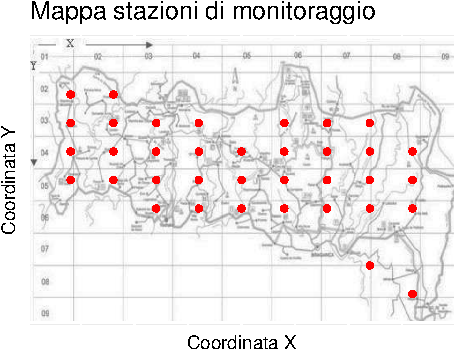
\includegraphics{ForestFires_files/figure-latex/mappa-1} \end{center}

Il dataset in esame contiene le seguenti variabili:

\begin{table}[H]
\centering
\caption{\label{tab:unnamed-chunk-1}Tabella variabili}
\centering
\begin{tabular}[t]{l|l}
\hline
Variabile & Descrizione\\
\hline
X & Coordinata X della stazione\\
\hline
Y & Coordinata Y della stazione\\
\hline
month & Mese della rilevazione\\
\hline
day & Giorno della settimana della rilevazione\\
\hline
FFMC & Codice FFMC (indica la secchezza del combustibile sottile)\\
\hline
DMC & Codice DMC (indica la secchezza del sottobosco)\\
\hline
DC & Codice DC (indica la secchezza degli strati organici profondi)\\
\hline
ISI & Indice di velocità iniziale\\
\hline
temp & Temperatura (in °C)\\
\hline
RH & Umidità relativa (in \%)\\
\hline
wind & Velocità del vento (in km/h)\\
\hline
rain & Pioggia (in mm/m²)\\
\hline
area & Area totale bruciata (in ha)\\
\hline
\end{tabular}
\end{table}

\begin{center}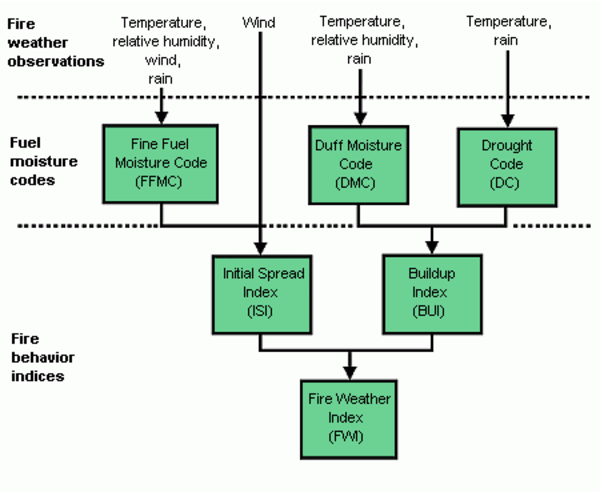
\includegraphics{ForestFires_files/figure-latex/unnamed-chunk-2-1} \end{center}

\end{document}
